\documentclass{standalone}
\usepackage{tikz}
\begin{document}
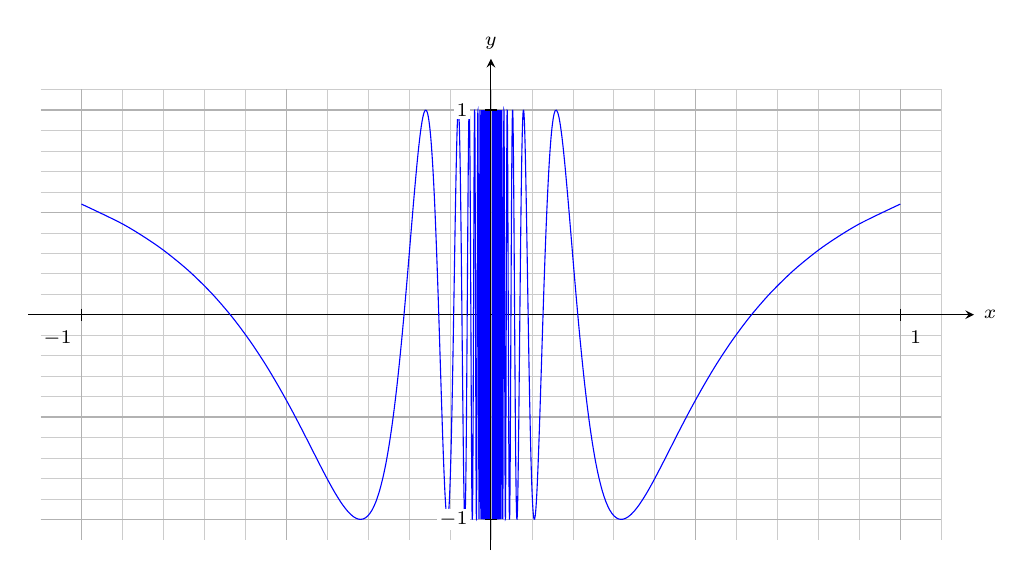
\begin{tikzpicture}[>=stealth, xscale=5.2, yscale=2.6]
  % Grid
  \draw[gray!40, very thin, step=0.1] (-1.1,-1.1) grid (1.1,1.1);
  \draw[gray!60, thin, step=0.5] (-1.1,-1.1) grid (1.1,1.1);
  % Axes
  \draw[->] (-1.13,0) -- (1.18,0) node[right, font=\scriptsize] {$x$};
  \draw[->] (0,-1.15) -- (0,1.25) node[above, font=\scriptsize] {$y$};
  % x-axis ticks and labels
  \draw (-1,0.03) -- (-1,-0.03) node[below left, font=\scriptsize] {$-1$};
  \draw (1,0.03) -- (1,-0.03) node[below right, font=\scriptsize] {$1$};
  % Curve: y = cos(1/x), oscillating infinitely often as x -> 0.
  % Parametrize by t = 1/x so samples concentrate near x = 0:
  %   x = 1/t, y = cos(t)  (t in radians), t from 1 to 280.
  % cos(1/x) is even, so mirror for x < 0.
  \begin{scope}
    \clip (-1.1,-1.05) rectangle (1.1,1.05);
    \draw[blue, line width=0.4pt, samples=2400, domain=1:280, variable=\t, smooth]
      plot ({1/\t}, {cos(\t r)});
    \draw[blue, line width=0.4pt, samples=2400, domain=1:280, variable=\t, smooth]
      plot ({-1/\t}, {cos(\t r)});
  \end{scope}
  % y-axis ticks and labels (drawn after the curve so the white
  % label backgrounds keep them legible over the dense oscillation)
  \draw (0.015,1) -- (-0.015,1)
    node[left=5pt, font=\scriptsize, fill=white, inner sep=1pt] {$1$};
  \draw (0.015,-1) -- (-0.015,-1)
    node[left=5pt, font=\scriptsize, fill=white, inner sep=1pt] {$-1$};
\end{tikzpicture}
\end{document}
